\chapter{Κρυπτογραφία}
\label{chapter:cryptography}

Στο κεφάλαιο αυτό θα γίνει μια εισαγωγή στην Κρυπτογραφία. Αρχικά θα αναλύσουμε βασικούς ορισμούς/μοντέλα κρυπτογραφικών σχημάτων, ξεκινώντας από πιο ιστορικούς και καταλήγοντας σε πιο σύγχρονους. Πολλοί από αυτούς θα χρησιμοποιηθούν στο Κεφάλαιο \ref{chapter:security} ως βασικά δομικά στοιχεία. Στη συνέχεια του κεφαλαίου θα αναλύσουμε κυρίως σύγχρονα κρυπτογραφικά εργαλεία και πρωτόκολλα που χρησιμοποιούνται ως συστατικά στοιχεία σε σύγχρονα πρωτόκολλα και πολλά από αυτά θα χρησιμοποιηθούν ως βασικά δομικά στοιχεία στα Κεφάλαια \ref{chapter:SMPC} και \ref{chapter:implementation}. Σε καμία περίπτωση αυτό το κεφάλαιο δεν αποτελεί μια πλήρη εισαγωγή στον κλάδο της κρυπτογραφίας. Ο αναγνώστης που ενδιαφέρεται για κάτι τέτοιο μπορεί να απευθυνθεί στα βιβλία \cite{boneh2020graduate}, \cite{hoffstein2008introduction}, \cite{pagourtzis2016computational}, το τελευταίο εκ των οποίων είναι και στην ελληνική γλώσσα.

\section{Βασικοί Ορισμοί}

\subsection{Πρωταρχικοί Ορισμοί}

Αρχικά θα αναφερθούμε στους πρώτους ιστορικά τυποποιημένους ορισμούς κρυπτογραφικών σχημάτων που έγιναν από τον Shannon, οι οποίοι αναφέρονται σε συστήματα συμμετρικής κρυπτογραφίας, με απώτερο σκοπό να μπορέσουμε να παρουσιάσουμε με σαφήνεια τα μοντέλα των αντιπάλων, της ασφάλειας και των αποδείξεων τους στην Ενότητα \ref{chapter:security}. Αυτά στη συνέχεια μπορούν να γενικευθούν, να προσαρμοστούν και να χρησιμοποιηθούν σε όλα τα κρυπτογραφικά κατασκευάσματα, όπως αυτά της ασύμμετρης κρυπτογραφίας, των συναρτήσεων κατακερματισμού, των κρυπτογραφικών πρωτοκόλλων κ.α.

Ο Shannon στην εργασία \cite{shannon1945mathematical} όρισε το παρακάτω γενικό μαθηματικό μοντέλο συμμετρικού κρυπτογραφικού σχήματος.

\begin{definition}
\label{def:shannon_cipher}
\textbf{Κρυπτογραφικό Σχήμα Shannon (Shannon Cipher)} : Ένα ζεύγος ντετερμινιστικών συναρτήσεων $\mathcal{E} = (\enc, \dec)$ οι οποίες ορίζονται ως εξής:
\begin{itemize}
    \item $\enc$ : $\mathcal{K} \times \mathcal{M} \rightarrow \mathcal{C}$
    \item $\dec$ : $\mathcal{K} \times \mathcal{C} \rightarrow \mathcal{M}$
\end{itemize}
όπου $\mathcal{M}$, $\mathcal{C}$, $\mathcal{K}$ είναι οι χώροι των μηνυμάτων, κρυπτοκειμένων και κλειδιών αντίστοιχα τους οποίους θα θεωρήσουμε πεπερασμένους. Στην περίπτωση αυτή λέμε ότι το κρυπτοσύστημα $\mathcal{E}$ ορίζεται πάνω στο $(\mathcal{K},\mathcal{M},\mathcal{C})$. Οι συναρτήσεις $\enc, \dec$ ορίζονται ως εξής:

\begin{itemize}
    \item H $\enc$ είναι η συνάρτηση κρυπτογράφησης και παίρνει ως όρισμα ένα κλειδί $k \in \mathcal{K}$ και ένα μήνυμα $k \in \mathcal{M}$ και επιστρέφει ένα κρυπτοκείμενο $c \in \mathcal{C}$. Δηλαδή :
    $$
    c = \enc_k(m) \text{ ή με ισοδύναμο συμβολισμό } c = \enc(k, m)
    $$
    \item H $\dec$ είναι η συνάρτηση αποκρυπτογράφησης, δηλαδή η αντίστροφη συνάρτηση της \enc, και παίρνει ως όρισμα ένα κλειδί $k \in \mathcal{K}$ και ένα κρυπτοκέιμενο  $c \in \mathcal{C}$ και επιστρέφει ένα μήνυμα $m \in \mathcal{M}$. Δηλαδή : 
    $$
    m = \dec_k(c) \text{ ή με ισοδύναμο συμβολισμό } m = \dec(k, c)
    $$
    %
\end{itemize}
    Όπου οι $\enc$, $\dec$ ακολουθούν την παρακάτω Ιδιότητα Ορθότητας:
    \begin{equation}
    \label{shannon_decryption_identity}
    \forall m \in \mathcal{M}, \forall k \in \mathcal{K} : Pr[m = \dec_k(\enc_k(m))] = 1
    \end{equation}
\end{definition}
{\setlength{\parindent}{0cm}
Ένα παράδειγμα Κρυπτογραφικού Σχήματος Shannon είναι αυτό του Σημειωματάριου Μιας Χρήσης (One Time Pad ή OTP) \cite{miller1882telegraphic} με σταθερό ή και μεταβλητό μήκος $m$ και $c$.
}

Δυστυχώς, ο Ορισμός \ref{def:shannon_cipher} είναι πολύ γενικός και η κλάση των κρυπτογραφικών σχημάτων που ορίζει, συμπεριλαμβάνει προβλήματα με μη πρακτικές χρονικές και χωρικές πολυπλοκότητες. Έτσι, υπήρξε ανάγκη στη βιβλιογραφία να συμπεριληφθεί μια ακόμα κλάση κρυπτογραφικών σχημάτων που εμπεριέχει, αποκλειστικά, κρυπτογραφικά σχήματα που μπορούν να υλοποιηθούν αποδοτικά.

\begin{definition}
\label{def:computational_cipher}
\textbf{Υπολογιστικό Κρυπτογραφικό Σχήμα (Computational Cipher) \cite{boneh2020graduate}} : Ένα ζεύγος συναρτήσεων $\mathcal{E} = (\enc, \dec)$ όπως ορίζονται στο Κρυπτογραφικό Σχήμα Shannon υπό τον περιορισμό ότι οι αλγόριθμοι $\enc$, $\dec$ είναι αποδοτικοί και πιθανοτικοί δηλαδή, $\enc, \dec \in PPT(\secparam)$, όπου $\secpar$ παράμετρος ασφάλειας, διατηρώντας την Ιδιότητα Ορθότητας \ref{shannon_decryption_identity}.
\end{definition}

Σήμερα για την ασφαλή ανταλλαγή μηνυμάτων διακρίνονται δύο κύριες κατηγορίες Υπολογιστικών Κρυπτογραφικών Σχημάτων. Τα Συμμετρικά και Ασύμμετρα Κρυπτογραφικά σχήματα, με τη λέξη "Υπολογιστικά" να παραλείπεται και να αναφέρεται μόνο όπου υπάρχει ανάγκη διάκρισης από άλλα σχήματα, αφού κυρίως μας ενδιαφέρουν πρακτικά σχήματα και σε αυτά θα επικεντρωθούμε και στα πλαίσια αυτής της εργασίας.

\subsection{Συμμετρική Κρυπτογραφία}

Η συμμετρική κρυπτογραφία παίρνει το όνομά της από τη συμμετρική χρήση κλειδιών, δηλαδή το ίδιο κλειδί που θα χρησιμοποιηθεί για την κρυπτογράφηση θα πρέπει να χρησιμοποιηθεί και για την αποκρυπτογράφηση. Στην κατηγορία των συμμετρικών κρυπτογραφικών σχημάτων ανήκουν τα περισσότερα σχήματα και συστήματα της Κλασσικής Κρυπτογραφίας.

\begin{definition}
\label{def:symetric_cryptographic_scheme}
\textbf{Συμμετρικό Κρυπτογραφικό Σχήμα (\EN{Symmetric Cryptographic \\ Scheme})} : Έστω κατάλληλα $\mathcal{M}$, $\mathcal{C}$, $\mathcal{K}$. Αποτελείτε από ένα σύνολο αποδοτικών αλγορίθμων $(\kgen, \enc, \dec)$ οι οποίοι ορίζονται παρόμοια με τον Ορισμό \ref{def:computational_cipher} και έχουν τις εξής λειτουργίες :
\begin{itemize}
    \item $k \leftarrow \kgen(1^\secpar)$ : Δημιουργεί ένα κρυπτογραφικό κλειδί $k$ το οποίο χρησιμοποιείται τόσο για κρυπτογράφηση όσο και για αποκρυπτογράφηση.
    \item $c \leftarrow \enc_{k}(m)$ : Κρυπτογραφεί ένα μήνυμα $m$ χρησιμοποιώντας το κλειδί $k$.
    \item $m \leftarrow \dec_{k}(c)$ : Αποκρυπτογραφεί ένα κρυπτοκείμενο $c$ χρησιμοποιώντας το κλειδί $k$.
\end{itemize}
Οι παραπάνω αλγόριθμοι πρέπει να ακολουθούν την εξής Ιδιότητα Ορθότητας όπως ακριβώς και με τον Ορισμό \ref{def:computational_cipher}.
\end{definition}

Ένα από τα βασικότερα μειονεκτήματα των συμμετρικών κρυπτογραφικών σχημάτων είναι ότι στην περίπτωση που χρησιμοποιούνται για ασφαλή επικοινωνία για κάθε συμμετέχοντα που θέλει να συμμετάσχει στην επικοινωνία θα πρέπει ο κάθε συμμετέχοντας να διαθέτει για την επικοινωνία τους ένα μοναδικό κλειδί. Δηλαδή στην περίπτωση των $n$ συμμετεχόντων θα χρειαστούμε $n^2$ κλειδιά, το πρόβλημα αυτό είναι γνωστό και ως Πρόβλημα των Τετραγώνων στη βιβλιογραφία. Έτσι τα σχήματα αυτά, από μόνα τους, καθίστανται ανίκανα για χρήση σε μεγάλα δίκτυα επικοινωνίας, όπως το Διαδίκτυο ή το Διαδίκτυο των Πραγμάτων. Ένα ακόμη μειονέκτημα είναι ότι οι συμμετέχοντες θα πρέπει να έχουν προαποφασίσει ένα συμμετρικό το συμμετρικό τους κλειδί. Τα προβλήματα αυτά έλυσε η εφεύρεση της ασύμμετρης κρυπτογραφίας. Τέλος σημαντικό είναι να αναφέρουμε ότι αυτά τα κρυπτογραφικά σχήματα λόγω του μεγάλου τους πλεονεκτήματος να έχουν πολύ γρήγορες υλοποιήσεις χρησιμοποιούνται κατά κόρον για μεταφορά μεγάλου όγκου δεδομένων.

\subsection{Ασύμμετρη Κρυπτογραφία}

Η ιστορία της Ασύμμετρης Κρυπτογραφίας αναφέρθηκε την Ενότητα \ref{chapter:intro}. Ο ορισμός των αντίστοιχων κρυπτογραφικών σχημάτων είναι παρόμοιος με αυτόν των συμμετρικών, με την κύρια διαφορά ότι υπάρχει ένα ζεύγος κλειδιών, το δημόσιο και το ιδιωτικό. Ο αυστηρώς ορισμός της παρουσιάζεται παρακάτω :

\begin{definition}
\label{def:assymetric_cryptographic_scheme}
\textbf{Ασυμμετρικό Κρυπτογραφικό Σχήμα (\EN{Assymetric Cryptographic \\ Scheme})} : Ορίζεται παρόμοια με τον Ορισμό \ref{def:symetric_cryptographic_scheme} με μοναδική διαφορά το ζέυγος κλειδιών και την ιδιότητα ορθότητας. Αποτελείτε από ένα σύνολο αλγορίθμων $(\kgen, \enc, \dec)$ με τις εξής λειτουργίες :
\begin{itemize}
    \item $(pk, sk) \leftarrow \kgen(1^\secpar)$ : Δημιουργεί ένα ζεύγος ασύμμετρων κρυπτογραφικά κλειδιών. Το Δημόσιο Κλειδί (Public Key) $pk$ που χρησιμοποιείται στην κρυπτογράφηση και το αντίστοιχο Ιδιωτικό Κλειδί (Private Key) $sk$ που χρησιμοποιείται στην αποκρυπτογράφηση.
    \item $c \leftarrow \enc_{pk}(m)$ : Κρυπτογραφεί ένα μήνυμα $m$ χρησιμοποιώντας το δημόσιο κλειδί $pk$.
    \item $m \leftarrow \dec_{sk}(c)$ : Αποκρυπτογραφεί ένα κρυπτοκείμενο $c$ χρησιμοποιώντας το ιδιωτικό κλειδί $sk$.
\end{itemize}
Όπως και στην περίπτωση της Συμμετρικής Κρυπτογραφίας οι παραπάνω αλγόριθμοι πρέπει να ακολουθούν την εξής ιδιότητα ορθότητας :
$$
    Pr(\dec_{sk}(\enc_{pk}(m))) = Pr(\enc_{sk}(\enc_{pk}(m))) = 1
$$
\end{definition}

Η τελευταία, ιδιότητα δηλαδή ότι $\dec_pk(m)=\enc^{-1}_sk(m)$ δίνει και την δυνατότητα για την υποστήριξη ψηφιακών υπογραφών και αποστολής μηνυμάτων με ένα ζεύγος κλειδιών ανά συμμετέχοντα.

Η Ασύμμετρη Κρυπτογραφία λύνει το πρόβλημα της διανομής κρυπτογραφικών κλειδιών που υπάρχει στην περίπτωση της Συμμετρικής, καθότι ο κάθε συμμετέχων χρειάζεται να διαθέτει μόνο ένα ζεύγος κλειδιών, από τα οποία το ένα μπορεί να το μοιραστεί δημόσια. Επίσης, μπορεί να χρησιμοποιηθεί ως συστατικό στοιχείο σε πολλά πρωτόκολλα με σκοπούς πέραν της απλής ανταλλαγής μηνυμάτων και των ψηφιακών υπογραφών, που θα ήταν αδύνατα χωρίς την ασύμμετρη κρυπτογραφία. Ωστόσο, αν και πρόκειται για σύγκριση ανόμοιων πραγμάτων, τα ασύμμετρα κρυπτογραφικά σχήματα είναι πιο κοστοβόρα (αρκετές δεκάδες φορές για μικρό μέγεθος μηνυμάτων και εώς και μια τάξη μεγέθους για μεγάλο μέγεθος μηνυμάτων) σε σχέση με τα συμμετρικά από άποψη υπολογισμών και πόρων στις υλοποιήσεις τους. Ένα απλό παράδειγμα φαίνεται στο Σχήμα \ref{code:rsa_vs_aes}\footnote{Είναι σημαντικό αναφέρουμε ότι σχεδόν όλοι οι σύγχρονοι CISC επεξεργαστές διαθέτουν εξειδικευμένα κυκλώματα καθώς και αντίστοιχες εντολές μηχανής και συμβολική γλώσσας για το κρυπτογραφικό σχήμα AES κάτι που σε καμία περίπτωση δεν ισχύει για τον RSA. Το τελευταίο οφείλεται και στο ότι η φύση τελευταίου δεν επιδέχεται μεγάλο βαθμό παραλληλοποίησης.} στο οποίο συγκρίνονται οι χρόνοι (cpu time) κρυπτογράφησης και αποκρυπτογράφησης ενός μικρού μηνύματος για τα σχήματα RSA και AES. Έτσι, σήμερα σε αρκετά δημοφιλή κρυπτογραφικά πρωτόκολλα, όπως για παράδειγμα στο πρωτόκολλο TLS \cite{RFC8446}, που χρησιμοποιείται για την ασφαλή επικοινωνία στο Επίπεδο Μεταφοράς ενός δικτύου, στην αρχή της συνεδρίας χρησιμοποιούνται ασύμμετρα σχήματα ψηφιακών υπογραφών και ανταλλαγής κλειδιών, όπως τα ECDSA και ECDHE αντίστοιχα, με σκοπό τη δημιουργία από κοινού συμμετρικών κλειδιών που χρησιμοποιούνται στη συνέχεια από συμμετρικούς αλγορίθμους για την κρυπτογράφηση των δεδομένων της επακόλουθης συνεδρίας. Ακόμα, ένα από τα κύρια χαρακτηριστικά των ασύμμετρων σχημάτων είναι η αυξημένη μαθηματική τους δόμηση. Αυτό έχει ως αποτέλεσμα συνήθως να βασίζονται έμμεσα σε πιο πολύπλοκους μαθηματικούς υπολογισμούς, όπως η εύρεση μεγάλων πρώτων αριθμών σε σχέση με τους σχετικά απλούς υπολογισμούς που εκτελεί ένα συμμετρικό σχήμα. Μια ακόμα συνέπεια του χαρακτηριστικού της αυξημένης μαθηματικής τους δόμησης, είναι ότι η ασφάλεια τους κατά κόρον βασίζεται σε υποθέσεις πολυπλοκότητας, όπως αυτές που θα αναφερθούν στην Κεφάλαιο \ref{chapter:security}, από τις οποίες πολλές από αυτές έχει αποδειχθεί ότι δεν ισχύουν σε μη κλασσικά μοντέλα υπολογισμού, όπως το κβαντικό \cite{shor1994algorithms}, αλλά και κάνουν την απόδειξη της ασφάλειας τους πιο πολύπλοκη.

\begin{figure}[h]
    \begin{center}
        \inputminted[fontsize=\scriptsize,frame=single]{python}{./01_body/code/rsa-vs-aes.py}
        \inputminted[fontsize=\scriptsize,frame=single]{text}{./01_body/code/rsa-vs-aes.output}
    \end{center}
    \caption{Μικρή σύγκριση των επιδόσεων για την κρυπτογράφηση και την αποκρυπτογράφηση ενός απλού μηνύματος μεταξύ συμμετρικών και ασύμμετρων κρυπτογραφικών σχημάτων (AES, RSA).}
    \label{code:rsa_vs_aes}
\end{figure}

\section{Κρυπτογραφικά Εργαλεία}

Στην Ενότητα αυτή θα μελετήσουμε σύγχρονα κρυπτογραφικά εργαλεία που αποτελούν βασικά συστατικά στοιχεία πολλών Κρυπτογραφικών Πρωτοκόλλων με διάφορες εφαρμογές. Πολλά από αυτά παρατηρούνται συχνά σε πρωτόκολλα SMPC κάτι που θα το παρατηρήσουμε πρακτικά και στο Κεφάλαιο \ref{chapter:SMPC}.

\subsection{Σχήματα Δέσμευσης (Commitment Schemes)}

Τα Σχήματα Δέσμευσης (Commitment Schemes) είναι το πρώτο εργαλείο που θα εξετάσουμε. Αυτά έχουν τη μορφή πρωτοκόλλων επικοινωνίας δύο φάσεων μεταξύ δύο (ή πιο σπάνια περισσότερων) συμμετεχόντων. Παρέχουν τη δυνατότητα σε έναν συμμετέχον, $S$, να δεσμευτεί κάποια συγκεκριμένη τιμή σε κάποιον άλλον, $R$, χωρίς όμως αυτός να γνωρίζει ο $S$ τη συγκεκριμένη τιμή, δηλαδή η τιμή είναι σε κρυπτογραφημένη μορφή. Το πρωτόκολλο δίνει τη δυνατότητα να αποκαλυφθεί στον $R$ η τιμή στην οποία δεσμεύτηκε αρχικά ο $V$, και μόνο αυτή, σε επόμενη χρονική στιγμή την οποία επιλέγει ο συμμετέχον $S$. Αυτό αποτρέπει τον συμμετέχον $S$ στο να μεταβάλλει την τιμή αυτή χωρίς να γίνει αντιληπτό από τον άλλο συμμετέχον. Τα σχήματα αυτά χρησιμοποιούνται ως δομικά στοιχεία σε σχήματα Αποδείξεων Μηδενικής Γνώσης αλλά και στον Ασφαλή Υπολογισμό. Το Σχήμα Δέσμευσης ορίζεται ως εξής :

\begin{definition}
    \textbf{Σχήματα Δέσμευσης} : Έστω $Μ$ ο χώρος των μηνυμάτων, $C$ ο χώρος των δεσμευμένων τιμών, $D$ ο χώρος των κλειδιών αποδέσμευσης και $R$ μια ομοιόμορφη πιθανοτική κατανομή που περιέχει αρκετή εντροπία για οποιοδήποτε σχήμα δέσμευσης. Τα σχήματα δέσμευσης είναι πρωτόκολλα δύο συμμετεχόντων, $S$ και $R$, στα οποία ο $S$ δεσμέυετε μια τιμή στον $R$. Αποτελούνται από μια τριάδα αλγορίθμων $(\text{Setup}, \text{Commit}, \text{Verify})$ που ορίζονται ως εξής :
    \begin{itemize}
        \item $\text{Setup}(\secparam)$ :
        \item $\text{Commit}(m, r)$ : Δέχεται ως όρισματα ένα μήνυμα $m$ και μερικά τυχαία νομίσματα $r$, και δίνει ως εξόδους μια δεσμευμένη τιμή $c$ και ένα κλειδί αποδέσμευσης $d$ για την $c$.
        \item $\text{Open}(c, m, d)$ : Δέχεται ως όρισματα μια δεσμευμένη τιμή $c$, το μήνυμα $m$ και το κλειδί ανοίγματος $d$, και δίνει ως έξοδο μια δυαδική τιμή ανάλογα με το αν η τιμή που φανερώθηκε από την αποδέσμευση της $c$ μέσω της $d$ είναι η $m$.
    \end{itemize}
    Το σχήμα πρέπει να ικανοποιεί τις παρακάτω ιδιότητες :
    \begin{itemize}
        \item \textbf{Ορθότητα (Completeness)} : $\forall m \in M, r \sample R : Pr[\text{Open}(\text{Commit}(m, r), m)] = 1$
        \item \textbf{Απόκρυψη (Hiding)} : $\forall \text{ distinct } m, m' \in M, r \sample \text{R}, \forall A :\\
         \abs{Pr[A(\text{Commit}(m, r))] - Pr[A(\text{Open(r, m')})]} \leq ε_h$
        \item \textbf{Δέσμευση (Binding)} : $\forall \text{ distinct } m, m', \forall \text{ distinct } d, d', \forall c :\\
         \abs{Pr[\text{Open}(c, m, d)] - Pr[\text{Open}(c, m', d')]} \leq ε_b$
    \end{itemize}
\end{definition}

Οι τιμές $ε_h$ και $ε_b$ εξαρτόνται από το είδος της ιδιότητας που θέλουμε να έχουμε. Σε αντιστοιχία με τους ορισμούς ασφάλειας αλλά και με την ισχύ του αντιπάλου που θα ορίσουμε στο επόμενο κεφάλαιο, μπορούμε να έχουμε \textbf{Υπολογιστική}, \textbf{Στατιστική} ή \textbf{Τέλεια} \textbf{Απόκρυψη} και \textbf{Δέσμευση} και οι τιμές που λαμβάνουν οι $ε_h$ και $ε_b$ είναι $0$, $negl(\secparam)$ και  $negl(\secparam)$ αντίστοιχα. Τέλος, μπορεί να αποδειχθεί σχετικά εύκολα, ότι δεν μπορούμε να έχουμε σχήματα που να διαθέτουν ταυτόχρονα τέλεια απόκρυψη και τέλεια δέσμευση.

\subsection{Αποδείξεις Μηδενικής Γνώσης}

Το επόμενο εργαλείο που θα εξετάσουμε είναι αυτό τον Αποδείξεων Μηδενικής Γνώσης. Η Μηδενική Γνώση είναι μια ιδιότητα που μπορεί να αποκτήσει η κλάση $\IP$ των Διαδραστικών Αποδείξεων αν υποθέσουμε ότι υπάρχουν Συναρτήσεις Μονής Διαδρομής (One Way Functions ή OWF), μια υπόθεση που θα δούμε στο επόμενο κεφάλαιο. Στο Κεφάλαιο \ref{chapter:appendix} κάνουμε μια μικρή μελέτη στις διαδραστικές αποδείξεις που είναι άμεσα συσχετισμένες με τις Αποδείξεις Μηδενικής Γνώσης. Διαισθητικά σε ένα πρωτόκολλο με την ιδιότητα αυτή ο Αποδεικνύων $P$, μπορεί να αποδείξει στον Επαληθευτή $V$ ότι γνωρίζει κάποιον μάρτυρα $w$ που ανήκει σε μια προκαθορισμένη γλώσσα $L$ που γνωρίζουν και οι δύο οντότητες, χωρίς ο $V$ να μπορεί να αποκτήσει γνώση σχετικά με τον $w$. Μια πιο παραστατική αντίληψη του πως λειτοργούν οι αποδείξεις με την ιδιότητα αυτή παρουσιάζεται στο Σχήμα \ref{fig:zero_knowledge_comic}. Σχετικά με τον αυστηρό ορισμό της ιδιότητας της Μηδενικής Γνώσης, χρειάστηκαν αρκετά χρόνια ώστε να υπάρξει ένας καταληκτικός ορισμός στη βιβλιογραφίας. Αυτός παρουσιάζεται παρακάτω σε αντιστοιχία με τον ορισμό της κλάσης IP:

\begin{figure}[ht]
    \centering
    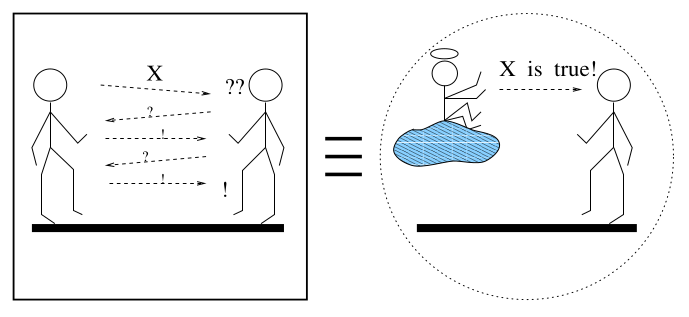
\includegraphics[width=10cm]{./01_body/images/zero_knowledge_comic.png}
    \caption{Κόμικ που αναπαρηστά πως λειτουργούν οι Αποδείξεις Μηδενικής Γνώσης \cite{goldreich2013short}.}
    \label{fig:zero_knowledge_comic}
\end{figure}

\begin{definition}
\label{def:czk}
\textbf{Κλάση Αποδείξεων Μηδενικής Γνώσης (\EN{Computational Zero Knowledge Proofs} ή $\CZK$)} : Έστω $P$ ντετερμινιστική συναρτήση ΤΜ που είναι απεριόριστης ισχύος. Η γλώσσα $L$ λέμε ότι ανήκει στην κλάση $\IP$, δηλαδή $L \in IP$ αν υπάρχει μη ντετερμινιστική ΤΜ $V$ με $x, r, a_{1}, \ldots, a_{i}, V$ και χρονική πολυπλοκότητα σε $O(poly(|x|))$ που ικανοποιεί τις παρακάτω ιδιότητες :s
\begin{itemize}
    \item \textbf{Πληρότητα (Completeness)} : $x \in L \Rightarrow \exists \operatorname{Pr}\left[\text { out }_{V}\langle V, P\rangle(x)=1\right] \geq (ε=) \dfrac{2}{3}$
    \item \textbf{Ορθότητα (Soundness)} : $x \notin L \Rightarrow \forall \operatorname{Pr}\left[\text { out }_{V}\langle V, P\rangle(x)=1\right] \leq 1 - ε$
    \item \textbf{Μηδενική Γνώση} : $\forall V, \exists S \in PPT : \forall x \in L \wedge w \in R_L$ :
    $$
    View_V = S(x,z)
    $$
\end{itemize}
\end{definition}

Προφανώς όπως ισχύει και για τις ιδιότητες της Πληρότητας και της Ορθότητας των Διαδραστικών Αποδείξεων έτσι και για την ιδιότητα της Μηδενικής Γνώσης μπορούμε να έχουμε από τους αντίστοιχους ορισμούς ασφάλειας που θα παρουσιαστούν στο επόμενο κεφάλαιο, \textbf{Τέλεια}, \textbf{Στατιστική} ή \textbf{Υπολογιστική Μηδενική Γνώση} ανάλογα με τον τύπο της δυσδιακριτότητας των κατανομών της μηδενικής γνώσης και οι κλάσεις που ορίζουν είναι οι $PZK$, $SZK$ και $CZK$ αντίστοιχα. Για τις κλάσεις αυτές γνωρίζουμε ότι $\PZK \subseteq \SZK \subseteq \CZK$. Η ευρύτερη από αυτές τις κλάσεις είναι αυτή της $\CZK$ που παρουσιάστηκε και στον Ορισμό \ref{def:czk}. Για την κλάση $\CZK$ γνωρίζουμε ότι $\IP=\CZK=\PSPACE$ και ότι $\NP \subseteq \CZK$, προφανώς υπό την υπόθεση OWF \cite{ben1988everything}. Για τις κλάσεις $\SZK$ και $\PZK$ ωστόσο δεν έχει αποδειχθεί κάποια παρόμοια ισότητα αλλά γνωρίζουμε το εξής $\PZK \subseteq \SZK \subseteq \AM \cap \coAM$ και επίσης εικάζεται ότι δεν ισχύει $NP \subseteq \SZK$ καθώς τότε καταρρέει όλη η πολυωνυμική ιεραρχία της $\NP$. Μια σύνοψη της γνώσης που έχουμε προς το παρόν για τις τρεις προηγούμενες κλάσεις, συμπεριλαμβανομένων και αρκετών σχέσεων που παραλήψαμε για λόγους συνοπτικότητας, μπορεί να βρεθεί στην εργασία \cite{couteau2017zero}. Δεν μπορούμε να παραλείψουμε να αναφέρουμε δύο σημαντικές κλάσεις που σχετίζονται άμεσα με την $CZK$, αυτή των Μη Διαδραστικών Αποδείξεων Μηδενικής Γνώσης, $NICZK$, και αυτή των Πιθανοτηκά Ελεγχόμενων Αποδείξεων $\PCP$, ωστόσο η μελέτη τους εμπείπτει εκτός τον σκοπώς αυτής της εργασίας.

Παρακάτω παρουσιάζεται ένα από τα πιο γνωστά σχήματα μηδενικής γνώσης, το Πρωτόκολλο Schnorr που μπορεί να χρησιμοποιηθεί για να αποδειχθεί η γνώση μιας λύσης ενός στιγμιοτύπου του προβλήματος του Διακριτού Λογαρίθμου, δηλαδή ενός στοιχείου $x$ τέτοιου ώστε $h=g^x$.

\begin{definition}
    \textbf{Πρωτόκολλο Schnorr : Απόδειξη Μηδενικής Γνώσης για τον Διακριτό Λογάριθμο} \cite{cramer1994proofs} :
    Έστω μια πολλαπλασιαστική ομάδα $G$, πρώτης τάξης με $\abs{G}=q$.
    \begin{itemize}
        \item \textbf{Εισόδοι} :
            \begin{itemize}
                \item $P$ : $x$, $h$
                \item $V$ : $h$
            \end{itemize}
        \item \textbf{Πρωτόκολλο} : 
            \pcb {
                P \< \< V \\ [][\hline]
                r \sample \mathbb{Z_q} \< \< \\
                u \gets g^r \< \< \\
                \< \sendmessageright*{u} \< \\
                \< \< c \sample \mathbb{Z}_q \\
                \< \sendmessageleft*{c} \< \\
                z \gets r + cx \< \< \\
                \< \sendmessageright*{z} \< \\
                \< \< g^z \stackrel{?}{=} u \cdot h^c
            }
        \item \textbf{Εξόδοι} :
            \begin{itemize}
                \item $P$ : $\perp$
                \item $V$ : $0$ ή $1$ ανάλογα με το αν ισχύει η τελευταία πράξη ισότητας που εκτέλεσαι
            \end{itemize}
    \end{itemize}
\end{definition}

\subsection{Σχήματα Ανυποψίαστης Μεταφοράς}

Τα σχήματα Ανυποψίαστης Μεταφοράς (Oblivious Transfer ή OT) είναι το επόμενο κρυπτογραφικό εργαλείο που θα μελετήσουμε.Πρόκειται πρωτόκολλα δύο συμμετεχόντων, $P_1$, $P_2$, στα οποία ο ένας συμμετέχον έχει $n$ τιμές και από τις οποίες ο άλλος συμμετέχον μπορεί να επιλέξει $t \le n$ από αυτές δίχως ο πρώτος συμμετέχον να γνωρίζει ποιες επέλεξε ο δεύτερος. Ίσως να ακούγεται ανόητη η χρησιμότητα τους όμως έχει αποδειχθεί ότι έχουν πολύ μεγάλη σημασία και δίχως σχήματα OT πολλά σύνθετα δεν μπορούν να υλοποιηθούν. Για να αντιληφθούμε την σημασία τους, έχει αποδειχθεί πως με βάση μόνο σχήματα OT μπορεί να υπολογιστεί οποιαδήποτε SMPC συνάρτηση \cite{10.1561/3300000019}. Το πρώτο πρωτόκολλο Ανυποψίαστης Μεταφοράς παρουσιάστηκε στην βιβλιογραφία το 1981 από τον Rabin, στην εργασία \cite{cryptoeprint:2005/187}. Μπορούμε να μοντελοποιήσουμε τα σχήματα αυτά ως εξης :

\begin{definition}
\textbf{Πρωτόκολλο Ανυποψίαστης Μεταφοράς t από τα n (Oblivious Transfer ή ΟΤ t-out-of-n)} :
\begin{itemize}
    \item \textbf{Εισόδοι} :
        \begin{itemize}
            \item $P_1$ : $b_{0}, b_{1}, \ldots b_{n} \in \bin^l$
            \item $P_2$ : $t_{0}, t_{1}, \ldots t_{n} \in \bin$
        \end{itemize}
    \item \textbf{Εξόδοι} :
        \begin{itemize}
            \item $P_1$ : $\perp$
            \item $P_2$ : \{$\forall t_n : b_{\{t_n = 1\}}\}$
        \end{itemize}
\end{itemize}
\end{definition}

Πολλές φορές στην βιβλιογραφία χρησιμοποιείται ο συμβολισμός OT t/n ή OT t-n, δηλαδή για παράδειγμα OT 1-2 ή OT 1/2. Παρακάτω παρουσιάζεται ένα πρωτόκολλο για OT 1-2 που είναι Σημασιολογικά Ασφαλές απέναντη σε Παθητικούς Αντιπάλους και παρουσιάστηκε στην εργασία \cite{even1985randomized}.

\begin{definition}
\label{def:oblivious_transfer}
\textbf{Πρωτόκολλο Ανυποψίαστης Μεταφοράς 1/2 (Oblivious Transfer 1/2)} \cite{even1985randomized} : 
\begin{itemize}
\item \textbf{Εισόδοι} : 
    \begin{itemize}
    \item Κοινή είσοδος : Οικογένεια Trapdoor Permutations (TDP) : $(I, S, F, F^{-1})$, Hardcore Predicate : $B$
    \item $P_{1}$ : $b_{0}, b_{1} \in\{0,1\}$
    \item $P_{2}$ : $\sigma \in\{0,1\}$.
    \end{itemize}
\item \textbf{Πρωτόκολλο} : \\
    \pcb {
    P_1 \< \< P_2 \\ [][\hline]
    (a, τ) \gets I(\secparam) \< \< \\
    \< \sendmessageright*{(a, t)} \> \\
    \< \< x_σ \gets S(a) \\
    \< \< y_{1-σ} \gets S(a) \\
    \< \< y_{σ} \gets F(a, x_s) \\
    \< \sendmessageleft*{y_0, y_1} \< \\
    x_0 \gets F^{-1}(a, y_0) \< \< \\
    x_1 \gets F^{-1}(a, y_1) \< \< \\
    β_0 \gets B(a, x_0) \oplus b_0 \< \< \\
    β_1 \gets B(a, x_1) \oplus b_1 \< \< \\
    \< \sendmessageright*{β_0, β_1} \< \\
    \< \< b_σ \gets B(a, x_σ) \oplus β_σ
    }

\item \textbf{Εξόδοι} :
    \begin{itemize}
        \item $P_1$ : $\perp$
        \item $P_{2}$ : $b_σ$
    \end{itemize}
\end{itemize}
\end{definition}

\subsection{Σχήματα Διαμοίρασης Μυστικών (Secret Sharing)}

Το τελευταίο κρυπτογραφικό εργαλείο που θα μελετήσουμε είναι αυτό των σχημάτων Διαμοίρασης Μυστικών. Για να αντιληφθούμε τη χρησιμότητα των σχημάτων Διαμοίρασης Μυστικών ας εξετάσουμε πρώτα ένα απλό παράδειγμα. Ας υποθέσουμε ότι ο ιδιοκτήτης μιας επιχείρησης έχει στην κατοχή του κάποια πολύ σημαντικά έγγραφα τα οποία βρίσκονται σε κάποια θυρίδα που είναι ασφαλισμένη με κάποιο κωδικό. Σε αυτά τα έγγραφα θέλει να έχει πρόσβαση το Διοικητικό Συμβούλιο της εταιρίας ακόμα και στην περίπτωση που αυτός δεν είναι παρόν, π.χ. στην περίπτωση που αυτός ξαφνικά φύγει από την ζωή, υπό την προϋπόθεση όμως ότι η πλεοψηφία, ή κάποιο συγκεκριμένο ποσοστό που έχει επιλέξει αυτός,των συμβούλων συμφωνεί στο άνοιγμα της θυρίδας. 

Το πρώτο κρυπτογραφικό σχήμα που λύνει το πρόβλημα αυτό παρουσιάστηκε από τον Shamir στην εργασία \cite{10.1145/359168.359176} το 1979 και σήμερα απαντάται στην βιβλιογραφία ως Πρωτόκολλο Διαμοίρασης Μυστικών Shamir. Βασίζεται στο γεγονός ότι οποιοδήποτε σύνολο $n+1$ σημείων σε ένα δυδιάστατο πεδίο $\mathbf{F}^2$ καθορίζει μοναδικά ένα πολυώνυμο $n$ βαθμού. Δηλαδή αν $f:\mathbb{F} \rightarrow \mathbb{F}$ όπου $f(x)=\pn{α}{x}$ τότε ένα σύνολο σημείων $(x_i, f(x_i))$ όπου $x \in [0, n]$ είναι επαρκές για να ανακτήσουμε την συνάρτηση $f$. Αυτό μπορεί πολύ εύκολα να συμβεί λύνοντας το σύστημα εξισώσεων μεγέθους $(n+1) \cdot (n+1)$ που προκύπτει αν αντικαταστήσουμε με κάθε σημείο την γενική εξίσωση πολυωνύμου $f(x_i)=\pn{a}{x_i}$. Ένας πιο εύκολος τρόπος να επιτευχθεί αυτό είναι μέσω των πολλαπλασιαστών Lagrange που αναλύθηκαν στην Ενότητα \ref{chapter:appendix}. Παρακάτω παρουσιάζονται οι δύο αλγόριθμοι του Πρωτοκόλλου Διαμοίρασης Μυστικών του Shamir, ένας για την διαμοίραση του μυστικού και ένας για την ανακατασκεύη του.

\begin{definition}
\textbf{Σχήμα Διαμοίρασης Μυστικών του Shamir (Shamir's Secret Sharing ή SSS)} : Έστω ένα πεδίο $\mathbb{F}$, $n$ παίκτες $P_0, P_1, P_2, \ldots, P_n$ που συμμετέχουν το πρωτόκολλο και μια τιμή $s \in \mathbb{F}$ που θα θεωρήσουμε ότι είναι το μυστικό που θέλει να διαμοιράσει ο παίκτης $P_0$, τον οποίο αποκαλούμε κάτοχο του μυστικού. Το πρωτόκολλο αυτό χρησιμοποιείται για την διαμοίραση  μυστικού σε $n$ συμμετέχοντες με τρόπο έτσι ώστε να χρειάζεται τουλάχιστον $t$, όπου $t \le n$, να συνεργαστούν ώστε να γίνει η αποκάλυψη του μυστικού.

\begin{itemize}
    \item \textbf{Πρωτόκολλο Διαμοίρασης} : Το πρωτόκολλο αυτό κτελείται μεταξύ όλων των συμμετεχόντων.
    \begin{itemize}
        \item \textbf{Εισόδοι} :
            \begin{itemize}
                \item Κοινή είσοδος : Πεδίο $\mathbb{F}$
                \item Κάτοχος του μυστικού $P_0$ : Μυστικό $s \in \mathbb{F}$
            \end{itemize}
        
        \item \textbf{Πρωτόκολλο} : \\
            \pcb {
                P_0 \< \< P_i\\ [][\hline]
                f(x) \sample \mathbb{F}[x] : deg(f_i(x)) = t+1 \land f_i(0) = s \< \< \\
                \forall i \in \{1, 2, \ldots\} : p_i \sample f(x)_{x \neq 0} \< \< \\
                \< \sendmessageright{top=$p_i$, bottom=to player $P_i$} \<
            }
        \item \textbf{Εξόδοι} : \\
            \begin{itemize}
                \item $P_i$ : $p_i$ (\textbf{Μετοχή του συμμετέχοντα } $i$)
            \end{itemize}
    \end{itemize}
    Το πρωτόκολλο ανακατασκευής εκτελείται μόνο μεταξύ των συμμετεχόντων που προσπαθούν να ανακατασκευάσουν το μυστικό $s$. Υποθέτουμε ότι μέσω κάποιου καναλιού επικοινωνίας τουλάχιστον $t+1$ από τους συμμετέχοντες συμμετέχοντες έχουν ανταλλάξει τα στοιχεία τους $p_i$ μεταξύ τους.
    \item \textbf{Πρωτόκολλο Ανακατασκευής} :
    \begin{itemize}
        \item \textbf{Εισόδοι} :
            \begin{itemize}
                \item Κοινή Είσοδος (των συμμετεχόντων που εκτελούν την ανακατασκευή): $S = \{\text{Σύνολο μετοχών } p_i \}$, όπου $t \le |S| \le n$
            \end{itemize}
        \item \textbf{Πρωτόκολλο} : \\
            \pcb {
                P_i \\ [][\hline]
                L(x) := \sum_{p_i \in S} p_i l_j(x) \textrm{, όπου } l_j(x) \textrm{ είναι οι συντελεστές Lagrange}\\
                s \gets L(0)
            }
        \item \textbf{Εξόδοι} :
            \begin{itemize}
                \item Κοινή Έξοδος : $s$
            \end{itemize}
    \end{itemize}
\end{itemize}

\end{definition}

Αξίζει να σημειωθεί ότι στην βιβλιογραφία έχουν προταθεί αρκετά πρωτόκολλα για Διαμοίραση Μυστικών. Όπως του Blakley \cite{blakley1979safeguarding}, του Mignotte και των Asmut-Bloom. Το πρώτο βασίζεται στο γεγονός ότι αν πάρουμε $n$ $n$-διάστατα υπερεπιπέδα με την προϋπόθεση ότι ανά δύο δεν είναι παράλληλα τότε όλα έχουν ένα κοινό μονοδιάστατο κοινό σημείο τομής. Έτσι αν θέλουμε να πάρουμε ένα σχήμα Διαμοίρασης Μυστικών με $n$ συμμετέχοντες και κατόφλι $t$, τότε αρκεί να δώσουμε ένα υπερεπίπεδο $t$-οστού βαθμού σε κάθε συμμετέχοντα, δηλαδή συνολικά $n$ υπερεπίπεδα υπό τον περιορισμό ότι όλα τα υπερεπίπεδα τέμνονται σε ένα σημείο το οποίο το επιλέγουμε εξ'αρχής και είναι ο μυστικό μας. Τέλος μια πολύ χρήσιμη ιδιότητα του σχήματος $SSS$ αλλά και αυτού του Blakley είναι ότι διαθέτουν τέλεια ασφάλεια, που εξηγούμε τι σημαίνει στο επόμενο κεφάλαιο. 